\documentclass{article}
\usepackage[T1]{fontenc}
\usepackage[utf8]{inputenc}
\usepackage{amsmath, amssymb}
\usepackage{tikz}
\usepackage{tikzsymbols}
\usepackage{lmodern}
\usepackage{xcolor}
\usetikzlibrary{arrows,automata}
\setlength\parindent{0pt}

\begin{document}

\begin{center}
  \Large{Informatik D - Übungsblatt 4}

  \large{Sebastian Höffner, Andrea Suckro}
\end{center}



\section*{Aufgabe 4.1}
Automat zur Addition zweier Binärzahlen.
\begin{center}
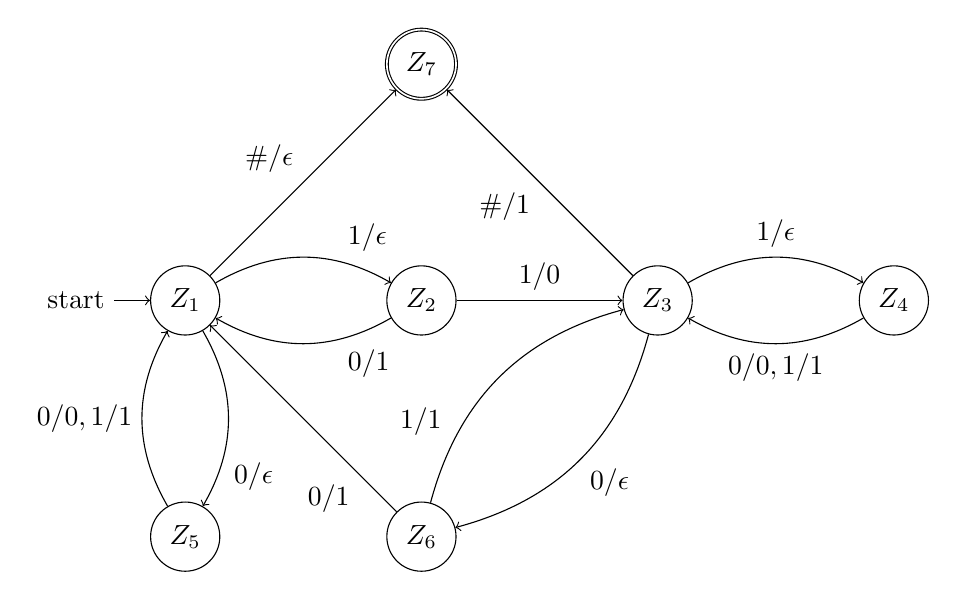
\begin{tikzpicture}[->, auto, node distance=3cm]
  \node[initial,state]   (Z1)               {$Z_1$};
  \node[state]           (Z2) [right of=Z1] {$Z_2$};
  \node[state]           (Z3) [right of=Z2] {$Z_3$};
  \node[state]           (Z4) [right of=Z3] {$Z_4$};
  \node[state]           (Z5) [below of=Z1] {$Z_5$};
  \node[state]           (Z6) [below of=Z2] {$Z_6$};
  \node[state,accepting] (Z7) [above of=Z2] {$Z_7$};

  \path (Z1) edge [bend left, pos=0.7] node {$0/\epsilon$} (Z5)
             edge [bend left, pos=0.7] node {$1/\epsilon$} (Z2)
             edge                      node {$\#/\epsilon$}(Z7)
        (Z2) edge [bend left, pos=0.3] node {$0/1$}        (Z1)
             edge                      node {$1/0$}        (Z3)
        (Z3) edge [bend left]          node {$0/\epsilon$} (Z6)
             edge [bend left]          node {$1/\epsilon$} (Z4)
             edge                      node {$\#/1$}       (Z7)
        (Z4) edge [bend left]          node {$0/0, 1/1$}   (Z3)
        (Z5) edge [bend left]          node {$0/0, 1/1$}   (Z1)
        (Z6) edge [pos=0.2]            node {$0/1$}        (Z1)
             edge [bend left, pos=0.2] node {$1/1$}        (Z3)
        ;
\end{tikzpicture}
\end{center}


\section*{Aufgabe 4.2}

\section*{Aufgabe 4.3}

\section*{Aufgabe 4.4}

\section*{Aufgabe 4.5}

\section*{Aufgabe 4.6}
Wenn die Sprache regulär ist, dann können wir z.B. einen endlichen Automaten oder regulären Ausdruck finden, der die Sprache $\mathbb{L} = \left\{a^ib^j | i \geq j \geq 0, j \leq 2000 \right\}$ beschreibt.

\subsection*{Regulärer Ausdruck}
In Übung 2 haben wir $\Smiley^x$ verwendet, um $x$ wiederholungen von $\Smiley$ darzustellen. Mit der gleichen Schreibweise können wir die Sprache $\mathbb{L}$ als regulären Ausdruck darstellen:

\begin{align*}
a^0a^*b^0|a^1a^*b^1|a^2a^*b^2|...|a^{2000}a^*b^{2000}
\end{align*}

\subsection*{NDEA}
Wir können die Sprache $\mathbb{L}$ auch als NDEA darstellen. Angenommen die Bedingung für $j$ ist nicht $j \leq 2000$ sondern $j \leq 0$, $j\leq 1$ oder $j \leq 2$.

Dann wären ein gültige Automaten:

$j \leq 0$:

\begin{center}
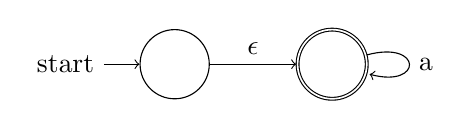
\begin{tikzpicture}[->, auto, node distance=2cm]
  \node[initial,state]   (Z1)               {};
  \node[state,accepting] (Z2) [right of=Z1] {};

  \path (Z1) edge              node {$\epsilon$} (Z2)
        (Z2) edge [loop right] node {a}          (Z2)
        ;
\end{tikzpicture}
\end{center}

$j \leq 1$:

\begin{center}
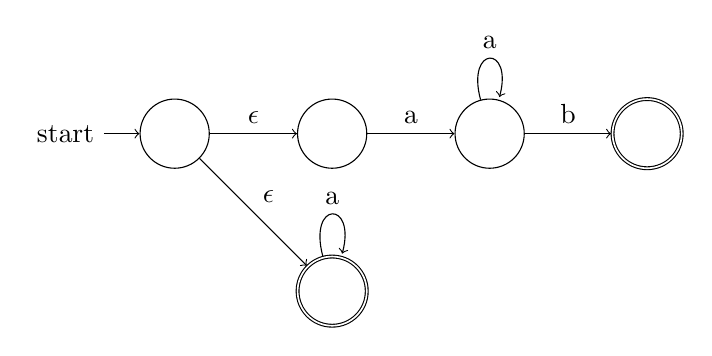
\begin{tikzpicture}[->, auto, node distance=2cm]
  \node[initial,state]   (Z1)               {};
  \node[state]           (Z2) [right of=Z1] {};
  \node[state,accepting] (Z3) [below of=Z2] {};
  \node[state]           (Z4) [right of=Z2] {};
  \node[state,accepting] (Z5) [right of=Z4] {};

  \path (Z1) edge              node {$\epsilon$} (Z2)
             edge              node {$\epsilon$} (Z3)
        (Z2) edge              node {a}          (Z4)
        (Z3) edge [loop above] node {a}          (Z3)
        (Z4) edge [loop above] node {a}          (Z4)
             edge              node {b}          (Z5)
        ;
\end{tikzpicture}
\end{center}

$j \leq 2$:

\begin{center}
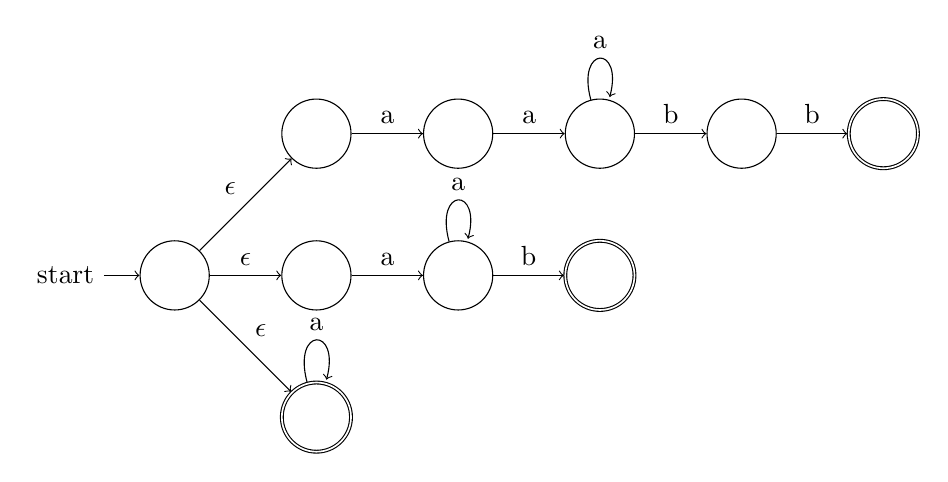
\begin{tikzpicture}[->, auto, node distance=1.8cm]
  \node[initial,state]    (Z1)               {};
  \node[state]            (Z2) [right of=Z1] {};
  \node[state,accepting]  (Z3) [below of=Z2] {};
  \node[state]            (Z4) [right of=Z2] {};
  \node[state,accepting]  (Z5) [right of=Z4] {};
  \node[state]            (Z6) [above of=Z2] {};
  \node[state]            (Z7) [right of=Z6] {};
  \node[state]            (Z8) [right of=Z7] {};
  \node[state]            (Z9) [right of=Z8] {};
  \node[state,accepting] (Z10) [right of=Z9] {};
  

  \path (Z1) edge              node {$\epsilon$} (Z2)
             edge              node {$\epsilon$} (Z3)
             edge              node {$\epsilon$} (Z6)
        (Z2) edge              node {a}          (Z4)
        (Z3) edge [loop above] node {a}          (Z3)
        (Z4) edge [loop above] node {a}          (Z4)
             edge              node {b}          (Z5)
        (Z6) edge              node {a}          (Z7) 
        (Z7) edge              node {a}          (Z8)
        (Z8) edge [loop above] node {a}          (Z8)
             edge              node {b}          (Z9) 
        (Z9) edge              node {b}          (Z10)
        ;
\end{tikzpicture}
\end{center}

Diesen Automaten können wir nach dem selben Schema erweitern, bis wir $j \leq 2000$ erfüllt haben.

\textbf{Die Sprache $\mathbb{L} = \left\{a^ib^j | i \geq j \geq 0, j \leq 2000 \right\}$ ist also regulär.}


\end{document}